\documentclass[11pt,a4paper]{article}
\usepackage[margin=2.1cm]{geometry}
\usepackage[utf8]{inputenc}
\usepackage[T1]{fontenc}
\usepackage{graphicx,booktabs,amsmath,amssymb,xcolor,microtype,longtable,array}
\usepackage{tikz}
\usetikzlibrary{arrows.meta,positioning,fit,backgrounds}
\usepackage[colorlinks=true,linkcolor=blue!60!black,citecolor=blue!60!black,urlcolor=blue!60!black]{hyperref}
\graphicspath{{../results/figures/}}

% Every number below is generated from results/*.csv by eval/plots.py ("TBD" = not run yet).
% Generated by eval/plots.py from results/*.csv - do not edit by hand
\newcommand{\numCorpusDocs}{24}
\newcommand{\numCorpusChunks}{1267}
\newcommand{\numCourses}{626}
\newcommand{\numFaculty}{339}
\newcommand{\numSlotRows}{70}
\newcommand{\numEvalQuestions}{30}
\newcommand{\numTotalRuns}{360}
\newcommand{\accMultiQwen}{94.4\%}
\newcommand{\refFMultiQwen}{0.95}
\newcommand{\falseRefMultiQwen}{4.8\%}
\newcommand{\citeRateMultiQwen}{100.0\%}
\newcommand{\correctSrcMultiQwen}{100.0\%}
\newcommand{\fabricatedMultiQwen}{3.6\%}
\newcommand{\routingMultiQwen}{100.0\%}
\newcommand{\latencyMultiQwen}{113.2}
\newcommand{\accMultiLlama}{82.2\%}
\newcommand{\refFMultiLlama}{0.93}
\newcommand{\falseRefMultiLlama}{4.8\%}
\newcommand{\citeRateMultiLlama}{83.6\%}
\newcommand{\correctSrcMultiLlama}{87.3\%}
\newcommand{\fabricatedMultiLlama}{0.0\%}
\newcommand{\routingMultiLlama}{98.9\%}
\newcommand{\latencyMultiLlama}{17.9}
\newcommand{\accSingleQwen}{92.2\%}
\newcommand{\refFSingleQwen}{0.90}
\newcommand{\falseRefSingleQwen}{9.5\%}
\newcommand{\citeRateSingleQwen}{91.2\%}
\newcommand{\correctSrcSingleQwen}{91.2\%}
\newcommand{\fabricatedSingleQwen}{1.8\%}
\newcommand{\routingSingleQwen}{n/a}
\newcommand{\latencySingleQwen}{96.0}
\newcommand{\accSingleLlama}{70.0\%}
\newcommand{\refFSingleLlama}{0.86}
\newcommand{\falseRefSingleLlama}{14.3\%}
\newcommand{\citeRateSingleLlama}{68.6\%}
\newcommand{\correctSrcSingleLlama}{88.2\%}
\newcommand{\fabricatedSingleLlama}{0.0\%}
\newcommand{\routingSingleLlama}{n/a}
\newcommand{\latencySingleLlama}{20.4}
\newcommand{\numQuestionsChanged}{9}

\newcommand{\todo}[1]{\textcolor{red}{\textbf{[TODO: #1]}}}

\title{\textbf{A Multi-Agent Academic Helpdesk for IIT Jodhpur}\\[2pt]
\large CSL7650 Autonomous Systems --- Assignment 2}
\author{\todo{team names and roll numbers}}
\date{October 2026}

\begin{document}
\maketitle

\begin{abstract}
We build a local, laptop-runnable academic helpdesk that answers questions about IIT Jodhpur programmes,
rules and regulations, course slots and the timetable, drafts (but never sends) e-mails to instructors,
cites the document every answer comes from, and refuses and logs questions it cannot answer.
The system uses Google ADK with 8B models served by Ollama (Qwen3-8B, Llama-3.1-8B) through LiteLLM,
retrieval-augmented generation over \numCorpusDocs{} institute documents (\numCorpusChunks{} chunks,
\texttt{nomic-embed-text} + ChromaDB) and deterministic tools over tables extracted from the official
slot-system and classroom-allocation PDFs. A single-agent baseline is compared with a multi-agent
organisation (an orchestrator delegating to Policy, Schedule and Email agents) on \numEvalQuestions{}
questions with repeated runs. The multi-agent system with Qwen3-8B reaches \accMultiQwen{} accuracy
(single agent: \accSingleQwen{}) and a refusal F1 of \refFMultiQwen{}.
The multi-agent organisation beats the single agent for both models, most strongly for the weaker
Llama-3.1-8B (\accMultiLlama{} vs.\ \accSingleLlama{}), and every configuration refuses all
out-of-scope questions; the remaining errors are concentrated in policy questions where an older
regulation conflicts with a later Senate circular.
\end{abstract}

%======================================================================
\section{Problem and environment}
The helpdesk must answer questions such as ``What is the attendance requirement to sit in the Major
exam?'', ``What is the slot for Autonomous Systems?'', ``How many 400-level electives has the Humanities
department floated this semester?'', ``How many Open Elective credits do I need for a B.Tech.?'' and
``Write an e-mail to the instructor of CSL7570 that I need leave for 2 days'', and must say it does not
know for questions such as ``What are the dining options on campus?''.

Using the environment properties from the course, the helpdesk's environment is
\emph{inaccessible} (the model sees only the retrieved passages, never the whole corpus),
\emph{non-deterministic} (sampling makes answers vary between runs --- ``from an agent's perspective even a
deterministic environment is non-deterministic'', which is why every question is run several times),
\emph{episodic} (questions are independent), \emph{dynamic} (rules, slots and office orders change outside
the agent; re-ingestion is how the system adapts) and \emph{discrete} (a finite set of routes and tools).

%======================================================================
\section{Design principles from the course}
Table~\ref{tab:principles} maps the concepts taught in class to concrete design decisions; the
subsections expand the most important ones.

\begin{table}[h]
\centering\small
\caption{Course concepts and where they appear in the system.}
\label{tab:principles}
\begin{tabular}{>{\raggedright\arraybackslash}p{5.2cm}>{\raggedright\arraybackslash}p{10.6cm}}
\toprule
Concept & Realisation in the helpdesk \\
\midrule
No full autonomy: constraints and guardrails & Scope governor, citation check, draft-only e-mail, escalation log \\
Effectoric capability; action pre-conditions & Each agent's tool set is its effectoric capability; an e-mail is drafted only after the instructor is resolved; an answer only after retrieval succeeds \\
Reactive vs.\ proactive balance; subsumption & A reactive keyword governor (highest-priority layer) subsumes deliberation for clearly off-topic questions; goal-directed agents handle the rest \\
BDI: \texttt{brf}, \texttt{options}, \texttt{filter}, \texttt{execute} & Retrieval updates beliefs; candidate routes are desires; the orchestrator's delegation is the intention; tool calls execute it; the pending e-mail persists across turns \\
Horizontal layering (mediator, $m^n$ bottleneck) vs.\ vertical two-pass & Delegation to one specialist instead of asking every agent and merging answers \\
Organisation-centric MAS: social, interaction, normative, communication structure & Roles (Table~\ref{tab:roles}); routing graph; norms (cite, do not guess, refuse and log); structured tool results and shared session state \\
Institutions: obligations, permissions, power; normative system $\langle E,F,G,C,\Delta\rangle$ & Per-role tool permissions; obligation to cite and to log; only humans close escalations (Sec.~\ref{sec:institution}) \\
Scenes, scene scripts, landmarks; trace & Query and e-mail scenes (Fig.~\ref{fig:arch}); every run is saved as an event trace \\
Coordination: blackboard, limited communication, scepticism, locally complete results & ADK session state is the blackboard; specialists only talk to the orchestrator; the citation guardrail does not trust uncited answers; specialists return final cited answers \\
Organisation adaptation (``emergent patterns become norms'') & The unanswered-question log is reviewed by humans, who add documents or rules \\
POMDP belief state; tiger problem (``listen'' before acting) & Retrieval scores are evidence; below the threshold the agent ``listens'' (asks, or refuses) rather than ``opens a door'' \\
ReAct / tool use & ADK's reason--act--observe loop with typed function tools \\
RAG and grounding & Chunked corpus, embeddings, threshold $\tau$, mandatory citations \\
Agent communication (speech acts, Contract-Net) & Delegation = \emph{request}, tool result = \emph{inform}, refusal = \emph{refuse}; Contract-Net bidding discussed as an alternative router \\
Argumentation & Resolving conflicting regulations by recency (Sec.~\ref{sec:argumentation}) \\
\bottomrule
\end{tabular}
\end{table}

\subsection{The helpdesk as an organisation}
We follow the organisation-centric view: the helpdesk is an entity whose heterogeneous agents together
fulfil one goal (correct, cited help), so no agent pursues a private goal. Roles are written in the
\emph{role description} format from class (objective, rights, norms), Table~\ref{tab:roles}. The
dependency type between orchestrator and specialists is \emph{delegate}.

\begin{table}[h]
\centering\small
\caption{Role descriptions (social structure).}
\label{tab:roles}
\begin{tabular}{>{\raggedright\arraybackslash}p{2.2cm}>{\raggedright\arraybackslash}p{4.0cm}>{\raggedright\arraybackslash}p{4.3cm}>{\raggedright\arraybackslash}p{4.2cm}}
\toprule
Role & Objective & Rights (tools) & Norms \\
\midrule
Orchestrator & Route each question to the right specialist & \texttt{transfer\_to\_agent}, \texttt{log\_unanswered} & Never answer academic questions itself; refuse and log non-academic ones \\
Policy agent & Answer questions on rules, regulations and curricula & \texttt{search\_documents}, \texttt{log\_unanswered} & Search first; cite every fact; prefer the most recent circular \\
Schedule agent & Answer slot, room, instructor and course-count questions & \texttt{get\_course\_info}, \texttt{get\_slot\_timing}, \texttt{list\_courses}, \texttt{search\_documents} & Never count by hand; cite the allocation/slot documents \\
Email agent & Draft e-mails to instructors & \texttt{get\_instructor\_email}, \texttt{draft\_email} & Never send; never invent reasons, dates or an instructor \\
Human (academic office) & Answer escalated questions & Reads \texttt{logs/unanswered.jsonl} & Closes escalations; adds documents \\
\bottomrule
\end{tabular}
\end{table}

\subsection{Institution and norms}\label{sec:institution}
The guardrails implement the institution's ``rules of the game''. With the normative system
$N=\langle E,F,G,C,\Delta\rangle$ from class: exogenous events are student messages; the generation
relation $G$ maps a message in state $X$ to institutional events --- \emph{answer}, \emph{refuse},
\emph{escalate}, or a violation $e\in E_{\mathit{violation}}$ (an off-topic request, or an answer that cites a
document never retrieved). The consequence relation $C$ adds fluents: a refusal adds the obligation fluent
\textit{obliged(human, answer(q))} (a line in \texttt{unanswered.jsonl}); a successful tool call adds the
domain fluent \textit{retrieved(doc)}, which the citation check later reads. Permissions are the per-role
tool sets (only the Email agent may create drafts); power to close an escalation belongs to humans only.
The ADK session state (``$s'$'') runs alongside the conversation (``$s$'').

\subsection{Conflicting documents as argumentation}\label{sec:argumentation}
The corpus contains a real conflict. The UG regulations (2019) say a student below 75\% attendance may
still sit the exams but needs at least a C grade; the Senate circular of 8 July 2024 says examination
performance is \emph{no longer linked} to attendance and ``supersedes the earlier policy in totality''.
As an abstract argumentation framework $\langle A,R\rangle$ with $A=\{a_{2019},a_{2024}\}$ and
$R=\{(a_{2024},a_{2019})\}$, the grounded extension is $\{a_{2024}\}$. The attack relation is stored
explicitly (a \texttt{supersedes} column in the manifest). When an amending circular and a regulation it
supersedes are retrieved together, \texttt{search\_documents} ranks the circular first and marks the older
passages as superseded. Without this, the first test run answered the attendance question from the 2019 rule,
even though the newer circular was among the retrieved passages and the prompt asked for the most recent document.

%======================================================================
\section{System}
\begin{figure}[h]
\centering
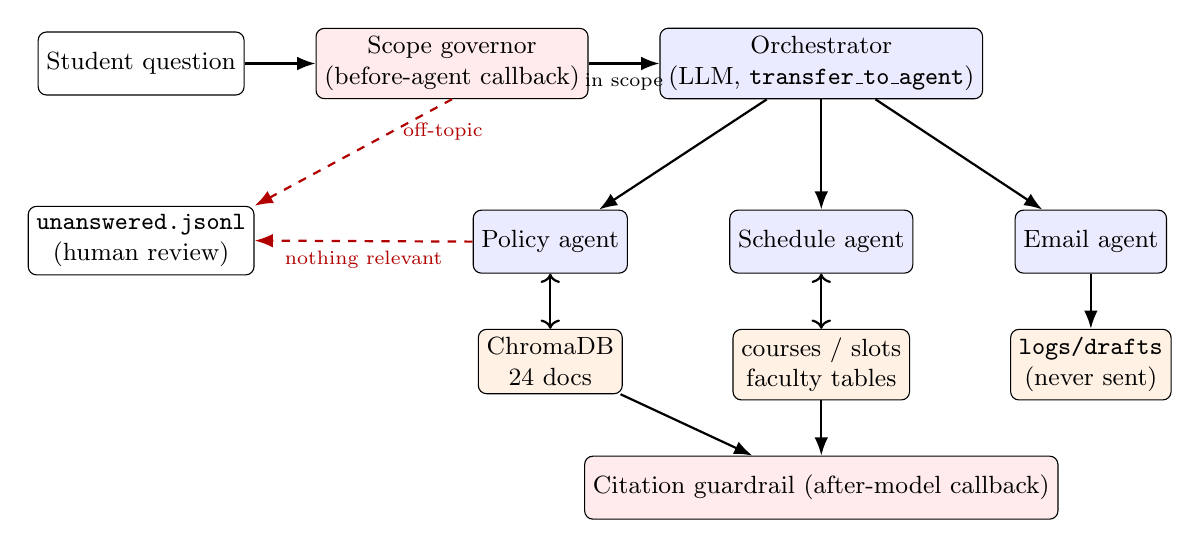
\begin{tikzpicture}[font=\small, node distance=6mm and 9mm,
  box/.style={draw, rounded corners=3pt, align=center, minimum height=8mm, inner sep=3pt},
  agent/.style={box, fill=blue!8}, store/.style={box, fill=orange!10}, gov/.style={box, fill=red!8},
  arr/.style={-{Latex}, thick}]
\node[box] (q) {Student question};
\node[gov, right=of q] (g) {Scope governor\\(before-agent callback)};
\node[agent, right=of g] (o) {Orchestrator\\(LLM, \texttt{transfer\_to\_agent})};
\node[agent, below left=14mm and 4mm of o] (p) {Policy agent};
\node[agent, below=14mm of o] (s) {Schedule agent};
\node[agent, below right=14mm and 4mm of o] (e) {Email agent};
\node[store, below=7mm of p] (c) {ChromaDB\\\numCorpusDocs{} docs};
\node[store, below=7mm of s] (t) {courses / slots\\faculty tables};
\node[store, below=7mm of e] (d) {\texttt{logs/drafts}\\(never sent)};
\node[gov, below=7mm of t] (cg) {Citation guardrail (after-model callback)};
\node[box, below=14mm of q] (log) {\texttt{unanswered.jsonl}\\(human review)};
\draw[arr] (q)--(g); \draw[arr] (g)--node[below,font=\scriptsize]{in scope}(o);
\draw[arr,dashed,red!70!black] (g.south)--node[right,font=\scriptsize,pos=0.3]{off-topic}(log.north east);
\draw[arr] (o)--(p); \draw[arr] (o)--(s); \draw[arr] (o)--(e);
\draw[arr,<->] (p)--(c); \draw[arr,<->] (s)--(t); \draw[arr] (e)--(d);
\draw[arr] (c)--(cg); \draw[arr] (t)--(cg);
\draw[arr,dashed,red!70!black] (p.west) -- node[below,font=\scriptsize]{nothing relevant}(log.east);
\end{tikzpicture}
\caption{Architecture. Dashed red arrows are refusals that are logged for a human.}
\label{fig:arch}
\end{figure}

\paragraph{Corpus.} \numCorpusDocs{} documents (listed in \texttt{ingest/manifest.csv}): UG, PG, M.Tech.,
M.S.\ (Research), Ph.D.\ and joint-programme regulations; the 2024 attendance and examination circulars
(scanned, OCR'd with Tesseract); continuation norms; the academic calendar AY 2026-27; the institute
statutes; curriculum pages for B.Tech.\ CSE/AIDE/EE; registration, minor/specialisation and programme-list
pages; the slot system and classroom allocation for Semester I 2026-27; a transcription of the slot
system's rules; and a faculty directory derived from the allocation with \emph{dummy} e-mail addresses
(personal data replaced, as allowed). PDFs are chunked per page, HTML/Markdown per section
(800 characters, 150 overlap) and embedded with \texttt{nomic-embed-text}.

\paragraph{Tables.} The classroom allocation PDF is parsed into \numCourses{} course offerings
(code, title, L-T-P, credits, slot, department, instructors, room, registrations, page) by reading words in
content-stream order (overflowing cells otherwise interleave characters) and splitting instructor cells at
backward jumps in $x$. The slot grid gives \numSlotRows{} (slot, day, time) rows and the faculty table
\numFaculty{} instructors. Because the PDF has no elective column, electives are \emph{inferred} from the
slot system's programme-wise allocation table (HSS courses at level $\ge$300 and courses in the elective
slots of their level); this is a documented heuristic.

\paragraph{Tools.} \texttt{search\_documents} (cosine distance threshold $\tau=0.35$, top-5, returns
\texttt{cite\_as} strings and document dates), \texttt{get\_course\_info}, \texttt{list\_courses} (exact
counts so the LLM never counts), \texttt{get\_slot\_timing}, \texttt{get\_instructor\_email},
\texttt{draft\_email} (saves a Markdown draft; never sends; only uses what the student said) and
\texttt{log\_unanswered}. Every tool records the documents it read in the session state.

\paragraph{Guardrails.} (1) The scope governor refuses clearly off-topic questions (dining, cab, weather,
cricket, \dots) before any LLM call; it is deliberately narrow, and anything it misses (e.g.\ ``best way to
reach the campus from the city'') must be refused by the agents themselves when retrieval finds nothing.
(2) The citation guardrail replaces an answer that cites a document no tool retrieved, or that was produced
without any tool, by a refusal and logs it; if the model used tools but forgot to cite, the retrieved
sources are attached and the run is flagged (``auto-attached'').

\paragraph{Threshold $\tau$.} On probe questions the best in-scope passage had cosine distance
$\le 0.26$ and out-of-scope questions $\ge 0.30$, but short keyword queries written by the agents reach
about $0.32$; we use $\tau=0.35$ and study 0.28 and 0.45 in the ablation.

%======================================================================
\section{Evaluation setup}
\numEvalQuestions{} questions (Appendix~\ref{app:questions}): 8 policy, 8 schedule, 5 e-mail, 6 out of scope
and 3 that sound academic but are not covered by the corpus; all five example questions from the
assignment are included. Gold answers were written from the documents and checked against them.
Configurations: \{multi-agent with LLM orchestrator, single agent\} $\times$ \{Qwen3-8B, Llama-3.1-8B\},
3 runs each at the models' default temperature, on an Intel i5-12450H laptop (CPU only, 16\,GB RAM).

Metrics: \emph{accuracy} (required facts present and no refusal; for questions that should be refused, a
refusal; automatic checks were verified by hand in \texttt{eval/human\_labels.csv});
\emph{refusal} precision/recall/F1 and false-refusal rate; over answered in-scope questions,
\emph{cited} (the model cited by itself), \emph{correct source} (a cited or attached document is a gold
source) and \emph{fabricated} (cites a document never retrieved); \emph{routing accuracy} (first specialist
the orchestrator delegated to); latency; and \emph{stability} --- questions whose outcome differs between runs.

%======================================================================
\section{Results}
% Generated by eval/plots.py from results/*.csv - do not edit by hand

\begin{table}[h]
\centering
\small
\caption{Main results (all runs). Citation columns are over answered in-scope questions; routing is the first specialist the orchestrator delegated to.}
\label{tab:main_results}
\resizebox{\ifdim\width>\linewidth\linewidth\else\width\fi}{!}{%
\begin{tabular}{lllrrrrrrrrr}
\toprule
System & Model & Router & Runs & Acc. & Ref.\ F1 & False ref. & Cited & Correct src. & Fabric. & Routing & Lat.\ (s) \\
\midrule
\multicolumn{12}{c}{\emph{Not run yet.}} \\
\bottomrule
\end{tabular}}
\end{table}

\begin{table}[h]
\centering
\small
\caption{Accuracy by question category.}
\label{tab:category}
\resizebox{\ifdim\width>\linewidth\linewidth\else\width\fi}{!}{%
\begin{tabular}{llrrrrr}
\toprule
System & Model & Policy & Schedule & Email & Out of scope & Uncovered \\
\midrule
\multicolumn{7}{c}{\emph{Not run yet.}} \\
\bottomrule
\end{tabular}}
\end{table}

\begin{table}[h]
\centering
\small
\caption{Questions whose outcome changed across repeated runs (correct in only some runs, or refused in only some runs).}
\label{tab:stability}
\resizebox{\ifdim\width>\linewidth\linewidth\else\width\fi}{!}{%
\begin{tabular}{lllllrr}
\toprule
Q & Category & System & Model & Correct & Refusal flip & Text sim. \\
\midrule
\multicolumn{7}{c}{\emph{Not run yet.}} \\
\bottomrule
\end{tabular}}
\end{table}

\begin{table}[h]
\centering
\small
\caption{Ablation (multi-agent, one run per question): guardrails switched off and retrieval threshold $\tau$ changed (default 0.35).}
\label{tab:ablation}
\resizebox{\ifdim\width>\linewidth\linewidth\else\width\fi}{!}{%
\begin{tabular}{lrrrrr}
\toprule
Configuration & Acc. & Ref.\ F1 & False ref. & Correct src. & Fabric. \\
\midrule
\multicolumn{6}{c}{\emph{Not run yet.}} \\
\bottomrule
\end{tabular}}
\end{table}


\begin{figure}[h]
\centering
\IfFileExists{../results/figures/accuracy_by_category.pdf}{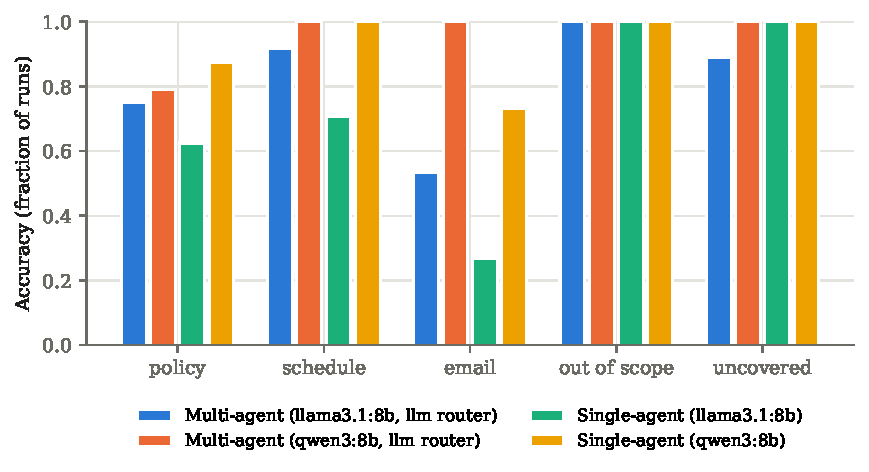
\includegraphics[width=0.75\linewidth]{accuracy_by_category.pdf}}{\fbox{figure generated after the evaluation run}}
\caption{Accuracy by question category.}
\end{figure}

Table~\ref{tab:main_results} gives the main comparison, Table~\ref{tab:category} the per-category accuracy,
Table~\ref{tab:stability} the questions whose answers changed across runs and Table~\ref{tab:ablation} the
ablation.

\paragraph{Single vs.\ multi agent.} With Qwen3-8B the two designs are close (\accMultiQwen{} vs.\
\accSingleQwen{}); the multi-agent system is better on citations (every cited document correct, against
\correctSrcSingleQwen{} for the single agent) and on false refusals. With Llama-3.1-8B the gap is large
(\accMultiLlama{} vs.\ \accSingleLlama{}); the single agent is weakest on the e-mail questions
(26.7\% against 53.3\% for the multi-agent system) and also lower on schedule and policy questions. We did not
test why; one plausible reason is that a specialist sees fewer tools and shorter instructions. Routing by the LLM orchestrator was almost always correct (\routingMultiQwen{} for Qwen,
\routingMultiLlama{} for Llama).

\paragraph{Qwen vs.\ Llama.} Qwen3-8B is more accurate and cites more reliably, but it is about six times
slower per question (113\,s against 18\,s for the multi-agent system), partly because it generates
reasoning before answering. Both models refuse every out-of-scope question in every run
(Table~\ref{tab:category}).

\paragraph{Where the systems fail.} The attendance question Q01 is answered incorrectly by all four
configurations. Qwen quotes the older rule from the 2019 regulations (a minimum C grade is needed below
75\%), although the 2024 Senate circular states that examination performance is no longer linked to
attendance. Llama gives the 75\% figure but does not say that the link was removed. This is exactly the
conflicting-regulations case that the system is meant to resolve: retrieval returns both documents and the
model does not prefer the later one. Q08 (credits for a minor) is another policy failure: Qwen's multi-agent
system answers 20 credits in two runs and 56 credits, citing the regulations portal, in the third.

\paragraph{Stability across runs.} Table~\ref{tab:stability} lists the questions whose outcome changed
between the three runs. Most are policy and schedule questions on Llama (for example Q04, Q08, Q10, Q15),
where the same question sometimes gets a correct answer and sometimes ``I don't know''. Qwen changed less:
Q03 and Q08 (multi-agent) and Q17 (both systems). Q17 asks for an e-mail to the instructor of CSL7570, a code
that is not in this semester's allocation; in some runs the system refuses with ``I don't know'' and in others it
asks the student to confirm the course code.

\paragraph{Ablation.} The ablation uses one run per question, so one question is 3.3 points and the
differences below are small. Removing the scope governor lowered accuracy from 96.7\% to 93.3\% and
correct-source rate to 94.7\%. Setting $\tau=0.28$ (stricter retrieval) lowered accuracy to 86.7\%, $\tau=0.45$ (looser)
gave 90.0\% and reduced refusal F1 from 0.95 to 0.82. We did not inspect individual runs to explain either change. Switching off the citation guardrail did
\emph{not} change accuracy, and the fabricated-citation rate was 0\% without it against 5.3\% with it, so
in this sample we cannot show that this guardrail helps; with so few questions that difference is one run.

\subsection{Example transcripts}
The following are verbatim outputs of the first multi-agent run.
% Generated by eval/plots.py from results/runs.csv - verbatim system output
\paragraph{Q09 (qwen3:8b).} \emph{What is the slot for the course Autonomous Systems?}\\
\textbf{Route:} HelpdeskOrchestrator $\rightarrow$ schedule\_agent\quad \textbf{Tools:} transfer\_to\_agent, get\_course\_info\quad \textbf{Latency:} 218\,s\\
\textbf{Answer:} The course Autonomous Systems (code: CSL7650) is offered in slot E [CLASS\_ALLOC\_2026, p.3].

\paragraph{Q10 (qwen3:8b).} \emph{How many 400 level electives have been floated by the Humanities department in this semester?}\\
\textbf{Route:} HelpdeskOrchestrator $\rightarrow$ schedule\_agent\quad \textbf{Tools:} transfer\_to\_agent, list\_courses\quad \textbf{Latency:} 162\,s\\
\textbf{Answer:} The Humanities department has floated 2 400-level elective courses this semester.  
Courses:  
1. LAL4070 (Health Economics)  
2. LAL4850 (Introduction to Climate Change Economics)  
Source: [CLASS\_ALLOC\_2026]

\paragraph{Q17 (qwen3:8b).} \emph{Write an email to the course instructor of CSL7570 that I need leave for 2 days}\\
\textbf{Route:} HelpdeskOrchestrator $\rightarrow$ email\_agent\quad \textbf{Tools:} transfer\_to\_agent, get\_instructor\_email\quad \textbf{Latency:} 133\,s\\
\textbf{Answer:} The course code CSL7570 was not found in the current semester's classroom allocation ([CLASS\_ALLOC\_2026](https://example.com/classalloc2026)), so its instructor cannot be determined. Please confirm the course code with your timetable or syllabus. Do not guess the instructor's email---use the correct code to proceed. 

[Cite: [FACULTY\_DIRECTORY] / [CLASS\_ALLOC\_2026]]

\paragraph{Q18 (qwen3:8b).} \emph{Write an email to the course instructor of CSL7650 that I need leave for 2 days due to fever on 14 and 15 October.}\\
\textbf{Route:} HelpdeskOrchestrator $\rightarrow$ email\_agent\quad \textbf{Tools:} transfer\_to\_agent, get\_instructor\_email, draft\_email\quad \textbf{Latency:} 204\,s\\
\textbf{Answer:} The draft email has been created and saved for review. Here's the draft:

Recipient: gaurav.harit@iitj-dummy.ac.in  
Subject: Request for leave of absence - CSL7650  
Body:  
Respected Professor Gaurav Harit,  

I am a student registered in CSL7650. I am writing to request leave of absence from the classes of this course.  

I need leave for 2 days due to fever on 14 and 15 October.  

I will cover the material taught during my absence. Kindly let me know if any supporting document is required.  

Thank you for your consideration.  

Yours sincerely,  
<Your Name>  
Roll No: <Roll No>  
IIT Jodhpur  

(!) Note: This is a draft and has NOT been sent. The email address is a dummy placeholder from [FACULTY\_DIRECTORY]. You must review and send it yourself.  

The draft is saved at: `logs/drafts/draft\_CSL7650\_20261026\_190335\_321654.md`  

Let me know if you need adjustments!

\paragraph{Q23 (qwen3:8b).} \emph{What is the best way to reach the campus from Jodhpur city center?}\\
\textbf{Route:} HelpdeskOrchestrator\quad \textbf{Tools:} log\_unanswered\quad \textbf{Latency:} 42\,s\\
\textbf{Answer:} I don't know. I can only answer questions about IIT Jodhpur academic programmes, rules and regulations, course slots and timetable, and draft e-mails to instructors.



%======================================================================
\section{Limitations}
\begin{itemize}
\item Retrieval-distance thresholds overlap between in-scope and out-of-scope questions; the final refusal
      decision relies on the LLM for borderline cases.
\item Elective status is inferred from slot rules; two of \numCourses{} allocation rows still contain
      merged text from overflowing PDF cells.
\item E-mail addresses are dummies; lab-slot durations are inferred from the grid layout.
\item Inference is slow for 8B models on a laptop (about 18\,s to 2\,min per question, run on an Apple M4
      with 16\,GB), which limits the number of runs to three per question and the ablation to one.
\item Correctness is labelled automatically with regular expressions against gold answers; we read a sample
      of borderline answers, but not all 360, so accuracy may be slightly misestimated.
\item With 30 questions and three runs, differences of a few points between configurations (especially in the
      ablation) are within noise.
\item The system cannot yet decide which of two conflicting regulations is newer and so should apply
      (Q01), and the weaker model sometimes refuses valid schedule questions.
\end{itemize}

\section{Group contributions}
\todo{who did what}

\begin{thebibliography}{9}
\bibitem{weiss} G.~Weiss (ed.). \emph{Multiagent Systems}, 2nd ed. MIT Press, 2013.
\bibitem{wooldridge} M.~Wooldridge. \emph{An Introduction to MultiAgent Systems}, 2nd ed. Wiley, 2009.
\bibitem{brooks} R.~Brooks. A robust layered control system for a mobile robot. \emph{IEEE J.\ Robotics and Automation}, 2(1), 1986.
\bibitem{bratman} M.~E.~Bratman. \emph{Intentions, Plans, and Practical Reason}. Harvard University Press, 1987.
\bibitem{dung} P.~M.~Dung. On the acceptability of arguments and its fundamental role in nonmonotonic reasoning, logic programming and n-person games. \emph{Artificial Intelligence}, 77(2), 1995.
\bibitem{react} S.~Yao et al. ReAct: Synergizing reasoning and acting in language models. ICLR 2023.
\bibitem{rag} P.~Lewis et al. Retrieval-augmented generation for knowledge-intensive NLP tasks. NeurIPS 2020.
\bibitem{fipa} FIPA. \emph{FIPA ACL Message Structure Specification} (SC00061G), 2002.
\end{thebibliography}

\appendix
\section{Question set}\label{app:questions}
% Generated by eval/plots.py from eval/questions.jsonl
\begin{small}
\begin{longtable}{>{\raggedright\arraybackslash}p{0.6cm}>{\raggedright\arraybackslash}p{1.4cm}>{\raggedright\arraybackslash}p{4.3cm}>{\raggedright\arraybackslash}p{5.6cm}>{\raggedright\arraybackslash}p{2.3cm}}
\toprule
ID & Category & Question & Expected answer / behaviour & Gold sources \\
\midrule
\endhead
Q01 & policy & What is the attendance requirement to sit in the Major exam? & Since the Senate amendment of 8 July 2024, examination performance is no longer linked to attendance, so there is no attendance cut-off for sitting the Major exam. Students are expected to attend fully; attendance should not fall below 75\%, and below 75\% without a valid reason the instructor can recommend de-registration from the course. & ATTEND\_\allowbreak{}POL\_\allowbreak{}2024 \\
Q02 & policy & How many Open Elective credits do I need to earn in order to get a B.Tech. Degree? & A regular B.Tech. requires 10 Open Elective (OE) credits (Table 11.2: OE = 10 of 150 graded credits; 0 for B.Tech. with specialization). & UG\_\allowbreak{}CREDIT\_\allowbreak{}TABLE, UG\_\allowbreak{}REG\_\allowbreak{}2019 \\
Q03 & policy & What is the minimum weightage and duration of the Major examination? & The Major examination is a 3-hour written exam with a weightage of not less than 40\% of the overall evaluation. & EXAM\_\allowbreak{}POL\_\allowbreak{}2024 \\
Q04 & policy & I missed my major exam because I was admitted to hospital. How do I apply for a make-up examination? & Apply to the Dean (Academics) through the course instructor within ten days of the missed exam, with the required medical certificate (hostel residents: certificate from the Institute Medical Officer). & UG\_\allowbreak{}REG\_\allowbreak{}2019, ACAD\_\allowbreak{}REG\_\allowbreak{}PORTAL \\
Q05 & policy & What is the maximum number of credits a UG student can register for in a semester? & A UG student may register for at most 25 credits in a semester (minimum 12). & UG\_\allowbreak{}REG\_\allowbreak{}2019, ACAD\_\allowbreak{}REG\_\allowbreak{}PORTAL \\
Q06 & policy & How many credits can I take during the summer term? & Students can register for summer courses up to a maximum of eight credits. & UG\_\allowbreak{}REG\_\allowbreak{}2019, ACAD\_\allowbreak{}REG\_\allowbreak{}PORTAL \\
Q07 & policy & What SGPA does an M.Tech. student need for continuation of assistantship? & SGPA 6.0 (for the first semester, >= 5); continuation in the programme needs CGPA 5.0 (2020 amendment). & CONTINUATION\_\allowbreak{}NORMS\_\allowbreak{}2020 \\
Q08 & policy & How many credits are needed for a minor or interdisciplinary specialization in B.Tech.? & 20 credits in the specialization/minor area: 10 can be counted as open electives and 10 are taken as course overload. & UG\_\allowbreak{}REG\_\allowbreak{}2019, SPEC\_\allowbreak{}MINOR\_\allowbreak{}RULES, ACAD\_\allowbreak{}REG\_\allowbreak{}PORTAL \\
Q09 & schedule & What is the slot for the course Autonomous Systems? & Autonomous Systems (CSL7650) is in slot E (Tue, Thu, Fri 11:00-11:50), room LHC 106. & CLASS\_\allowbreak{}ALLOC\_\allowbreak{}2026 \\
Q10 & schedule & How many 400 level electives have been floated by the Humanities department in this semester? & Two: LAL4070 Health Economics and LAL4850 Introduction to Climate Change Economics (School of Liberal Arts). & CLASS\_\allowbreak{}ALLOC\_\allowbreak{}2026 \\
Q11 & schedule & What are the lecture days and timings for Slot E? & Slot E meets Tuesday, Thursday and Friday, 11:00-11:50. & SLOT\_\allowbreak{}SYS\_\allowbreak{}2026 \\
Q12 & schedule & Who is the instructor for Database Systems and in which classroom does it meet? & Database Systems (CSL3050) is taught by Awathare Nitin Niranjan in LHC 2 101 (slot A). & CLASS\_\allowbreak{}ALLOC\_\allowbreak{}2026 \\
Q13 & schedule & Who teaches Digital Fabrication and what is its course code? & Digital Fabrication is MEL3050, taught by Gopal Dnyanba Gote (slot A, LHC 205). & CLASS\_\allowbreak{}ALLOC\_\allowbreak{}2026 \\
Q14 & schedule & What is the maximum number of students per lab and per tutorial in the slot system? & Maximum 50 students per lab and about 40 per tutorial. & SLOT\_\allowbreak{}SYS\_\allowbreak{}2026, SLOT\_\allowbreak{}SYS\_\allowbreak{}RULES\_\allowbreak{}2026 \\
Q15 & schedule & Which slots are used for compulsory courses of UG 2nd year students? & A-E for programme compulsory courses, U for institute electives, and K \& N for programme compulsory courses if the strength is below 160. & SLOT\_\allowbreak{}SYS\_\allowbreak{}2026, SLOT\_\allowbreak{}SYS\_\allowbreak{}RULES\_\allowbreak{}2026 \\
Q16 & schedule & In which slot and room is Database Systems, and on which days does that slot meet? & CSL3050 Database Systems is in slot A, LHC 2 101; slot A meets Monday, Tuesday and Thursday 09:00-09:50. & CLASS\_\allowbreak{}ALLOC\_\allowbreak{}2026, SLOT\_\allowbreak{}SYS\_\allowbreak{}2026 \\
Q17 & email & Write an email to the course instructor of CSL7570 that I need leave for 2 days & CSL7570 is not in the AY 2026-27 Sem I classroom allocation, so the agent must not invent an instructor; it should say the code was not found and ask the student to confirm it (Autonomous Systems is CSL7650). & CLASS\_\allowbreak{}ALLOC\_\allowbreak{}2026 \\
Q18 & email & Write an email to the course instructor of CSL7650 that I need leave for 2 days due to fever on 14 and 15 October. & Draft (not sent) to Gaurav Harit, gaurav.harit@iitj-dummy.ac.in, requesting leave for 14-15 October due to fever. & FACULTY\_\allowbreak{}DIRECTORY \\
Q19 & email & Draft an email to the instructor of CSL3050 asking for a make-up exam because I missed the minor exam on 20 September due to hospital admission. & Draft (not sent) to awathare.nitin.niranjan@iitj-dummy.ac.in requesting a make-up for the minor exam missed on 20 September. & FACULTY\_\allowbreak{}DIRECTORY \\
Q20 & email & Draft an email to the instructor of MEL2060 asking about the syllabus for the upcoming quiz. & Draft (not sent) to rajit.ranjan@iitj-dummy.ac.in asking about the quiz syllabus. & FACULTY\_\allowbreak{}DIRECTORY \\
Q21 & email & I need an email drafted to my instructor for a medical absence. & No course is given, so the agent should ask which course (course code) the e-mail is for instead of drafting one. & -- \\
Q22 & out of scope & What are the available dining options on the campus? & Refuse ('I don't know') and log the question for a human. & -- \\
Q23 & out of scope & What is the best way to reach the campus from Jodhpur city center? & Refuse ('I don't know') and log the question for a human. & -- \\
Q24 & out of scope & What is the weather forecast for Jodhpur this weekend? & Refuse ('I don't know') and log the question for a human. & -- \\
Q25 & out of scope & Who won the cricket world cup? & Refuse ('I don't know') and log the question for a human. & -- \\
Q26 & out of scope & Which movies are showing at the mall in Jodhpur? & Refuse ('I don't know') and log the question for a human. & -- \\
Q27 & out of scope & Can you write a python script to scrape data from twitter? & Refuse ('I don't know') and log the question for a human. & -- \\
Q28 & uncovered & What is the policy for swimming pool access and coach timings for B.Tech students? & Not covered by the documents: say 'I don't know' and log the question. & -- \\
Q29 & uncovered & What is the mess fee refund policy if I am on leave for 15 days? & Not covered by the documents: say 'I don't know' and log the question. & -- \\
Q30 & uncovered & What are the rules and stipend for the 2029 quantum technology exchange fellowship? & Not covered by the documents: say 'I don't know' and log the question. & -- \\
\bottomrule
\end{longtable}
\end{small}


\section{Reproduction}
\begin{verbatim}
uv venv --python 3.12 && uv pip install -r requirements.txt
ollama pull qwen3:8b && ollama pull llama3.1:8b && ollama pull nomic-embed-text
python main.py ingest --rebuild
python -m pytest -q
python eval/run_eval.py                      # full grid
python eval/run_eval.py --ablation --model qwen3:8b
python eval/run_eval.py --score-only         # after editing eval/human_labels.csv
cd report && pdflatex report.tex && pdflatex report.tex
\end{verbatim}
\end{document}
